\documentclass[12pt, a4paper]{article}
\usepackage[UTF8]{ctex}
\usepackage{amsmath}
\usepackage{amssymb}
\usepackage{amsthm}
\usepackage{geometry}
\usepackage{enumitem}
\usepackage{indentfirst}
\usepackage{caption}
\usepackage{fancyhdr}
\usepackage{booktabs}
\usepackage{titlesec}
\usepackage{draftwatermark}
\usepackage{graphicx} % 导入图像的宏包、单图





% 页面布局设置
\geometry{top=2.54cm, bottom=2.54cm, left=3.18cm, right=3.18cm}

% 行距设置
\linespread{1.5}

%设置水印
\SetWatermarkText{B站：布加拉提}
\SetWatermarkScale{0.4}
% 段落设置
\setlength{\parindent}{2em}
\setlength{\parskip}{0.5em}

% 节标题格式设置
\titleformat{\section}{\normalfont\Large\bfseries}{第\chinese{section}章、}{1em}{}
\titlespacing{\section}{0pt}{2.5ex plus 1ex minus .2ex}{1.3ex plus .2ex}

% 定理环境设置
\newtheoremstyle{solution}
{}
{}
{}
{}
{\bfseries}
{、}
{1em}
{}
\theoremstyle{solution}
\newtheorem{sol}{解}

% 页眉页脚设置
\pagestyle{fancy}
\fancyhf{}
\fancyhead[C]{b站布加拉提整理（回忆版）b站甘茶w独家讲解}
\fancyfoot[C]{\thepage}

\rfoot{整理人：八方\\资源提供：考研乔瑟夫}
\lhead{
\includegraphics[width=0.06\linewidth]{p1.png}}
\rhead{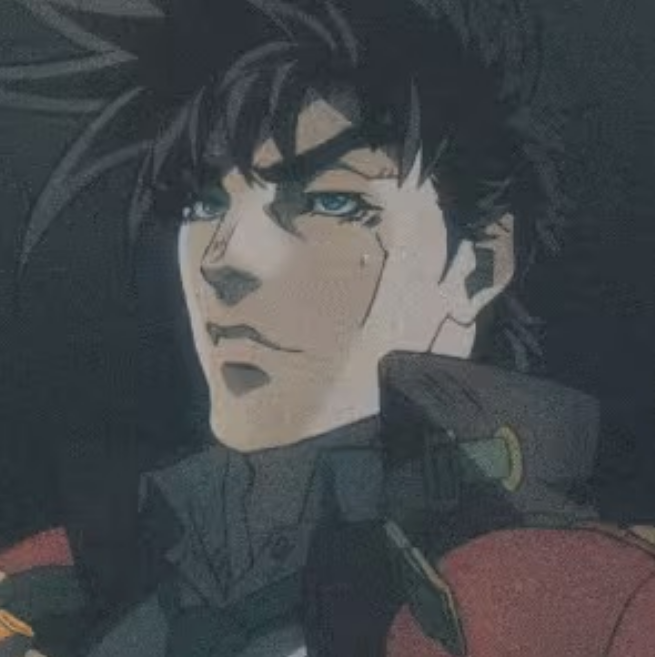
\includegraphics[width=0.06\linewidth]{p2.png}}
\renewcommand{\headrulewidth}{0.4pt}
\renewcommand{\footrulewidth}{0.4pt}

\begin{document}

\begin{center}
\Large\textbf{2009哈工大硕士考试试题：805物理光学}
\end{center}




\section*{一、填空与选择（28分）}
\begin{enumerate}
    \item 发生全发射条件为\_\_\_\_\_,\_\_\_\_\_,全反射现象的特点为\_\_\_\_\_,\_\_\_\_\_,和\_\_\_\_\_。
    \item 光源的时间相干性可用\_\_\_\_\_,\_\_\_\_\_和\_\_\_\_\_三个任意量的任意一个来表征。
    \item \_\_\_\_\_\_\_\_\_\_叫波阵面。
    \item 法布里-波罗干涉仪利用平板的\_\_\_\_\_工作原理。
    \item 在相干照明的情况下，平行平板产生\_\_\_\_\_干涉；楔形平板产生\_\_\_\_\_干涉。
    \item 影响干涉条纹对比度的因素有\_\_\_\_\_,\_\_\_\_\_和\_\_\_\_\_。
    \item 根据瑞利判据，望远镜的分辨率为\_\_\_\_\_,照相机物镜的分辨率为\_\_\_\_\_,显微镜物镜的分辨率为\_\_\_\_\_。
    \item 三个理想偏振片堆叠起来，每片通过光轴相对前一片都顺时针旋转$30^\circ$,光强为$I_0$的非偏振光入射。穿过偏振片堆后，光强为\_\_\_\_\_。
    \item 光在界面上的反射与透射特性由\_\_\_\_\_，\_\_\_\_\_和\_\_\_\_\_三个因素决定。
    \item （重复）真空中传播的平面电磁波，其电场表达式为$E_x=0,E_y=0,E_z=(10^2V/m)cos[\pi\times10^{14}s^{-1}(t-x/c)+\pi/2]$,该电磁波的频率，波长为\_\_\_\_\_，周期为\_\_\_\_\_，振幅为\_\_\_\_\_，初相位为\_\_\_\_\_.
    \item 观察屏距离衍射屏优先远的衍射称为\_\_\_\_\_，观察屏距离衍射屏无限远的衍射称为\_\_\_\_\_。
    \item （重复）假设某一介质对空气的临界角是60°，则光从空气射向此介质时的布儒斯特角是\_\_\_\_\_.\\(A)$tg^{-1}\sqrt({3}/2)$\qquad(B)$tg^{-1}(1/2)$\qquad(C)$tg^{-1}(2\sqrt{3}/3)$\qquad(D)$tg^{-1}2$
    \item 产生光电效应的本质原因是\_\_\_\_\_.\\(A)电场对光场的直接影响\qquad(B)电场对介质性质的直接影响\qquad(C)其他因素
    \item （重复）在真空中波长为$\lambda$ 的单色光，再折射率为$n$ 的透明介质中从A传播到B，若A,B两点的相位差为3\(\pi\) ,则此路径AB地光程差为\_\_\_\_\_.\\(A)1.5\(\lambda\) \qquad(B)1.5\(n\lambda\) \qquad(C)3\(\lambda\) \qquad(D)1.5\(\lambda/n\)
    \item （重复）在夫琅和费单缝衍射实验中，对于给定的入射单色光，当缝宽变小时，除中央亮纹位置不变，各级衍射条纹\_\_\_\_\_.\\(A) 对应的衍射角变小\\(B) 对应的衍射角变大\\（C）对应的衍射角不变\\（D）光强也不变
\end{enumerate}
\section*{二、解释下列名词}
\begin{enumerate}
    \item 巴比涅原理
    \item 半波损失
    \item 艾里斑
    \item 相速度
    \item 磁光效应
    \item 双折射
    \item 条纹对比度
    \item 古斯-哈思斯位移
\end{enumerate}
\section*{三、简答题}
\begin{enumerate}
    \item 什么是空间频率，它的物理意义是什么？
    \item 根据波动理论，简述平面波和球面波的区别。
    \item 以杨氏双缝干涉实验为例，简述光波干涉与衍射的关系。
    \item 什么是光栅方程？简述它的物理意义。
    \item 比较棱镜与光栅的色分辨本领的差异。
\end{enumerate}
\section*{四、计算题}
\begin{enumerate}
    \item 两束相干平面波在$yz$平面传播，其传播方向与$z$轴夹角分别为30°和-30°，求$y$轴上干涉光强分布及条纹间距。
    \item （重复）夜间，在一棵人造卫星拍地球的照片。如果所用照相机镜头的焦距为50$mm$,$F$数为2，试问在100$km$以外能否分辨开汽车上的两盏灯（假定车灯间距为2000$mm$，中心波长$500nm$）?
    \item （重复） 以纳光观察迈克尔逊干涉条纹，先看到干涉场中12个亮环，且中心是亮点，然后移动一侧反射镜，看到中心消失了10个亮环，此时干涉场中还存在5个亮环。求：
    \begin{enumerate}
        \item 镜面移动的距离
        \item 开始时中心亮斑的级次$k_0$,相对应的等效空气薄膜厚$h_0$
    \end{enumerate}
    \item 通过偏振片观察部分偏振光时，当偏振片绕入射光方向转到某位置上，投射光强为极大，然后再将偏振片旋转30度发现投射光强为极大值的7/8，试求该入射部分偏振光的偏振度P及该光内自然光与线偏振光强之比。
\end{enumerate}
\section*{五、综合题}
\begin{enumerate}
    \item 请画出迈克尔逊干涉仪的工作原理，说明它可能有说明用途，根据你的理解，讨论其时间相干性，当光源分别为点光源和扩展光源时，讨论干涉条纹定义域。

\end{enumerate}
\end{document}